\chapter{Real-time Processing in the Big Data Context}
\label{chap:real_time_processing}

Many information systems require today fast or even instant response to a coming data.
When new piece of data arrives into the system from a user, sensor, or any other outer source, system must reflect changes of its state quickly. 
The batch processing, that we describe in the Chapter~\ref{chap:google_architecture}, cannot fulfil this requirement, because it takes usually long time to execute.
The real-time processing allows doing that.

Necessity of response to a coming data fast is especially applicable to the Web world.
Companies like Google, Twitter, LinkedIn, Facebook, etc. process not just much of data, but also often need to do it quickly.
This, in fact, brings to a simultaneous use of both types of processing in one system.

We already described the batch processing and the MapReduce paradigm as its application.
It has two considerable advantages.
First of all, it is very efficient.
It fetches batches of data, and processes them at once, what is always faster, than taking records arbitrarily one by one.
Another advantage is that it allows execution on data of any function we have in mind, as long as all data is at the disposal.
When we have data coming from the stream record by record, this is not possible.
In that case we have to create alternative methods to apply the same algorithms.
Usually they become approximated, and accuracy is a matter of tradeoff.

To define the real-time processing, we need first to explain what the real time is.
There is no such thing in physics as real time, because any event takes time to happen.
But human understands, and even feels, that one event takes long time, but another is happening ``instantly''.
This is of course only a matter of our perception.
We are not able to differentiate intervals smaller than fractions of second.
As a result, we define real time as an interval of time that short enough in the current context.
In some cases it is seconds or minutes, but sometimes even milliseconds, and then things become really interesting.

The real-time processing is then processing of the data that takes time, short enough in the current context.
Let us consider two examples.
The first is a page visits counter.
It does not require any super-fast reflection of how many people visited the page, and as a result, system can update it once in a minute, aggregating all visit events during this time.
Real time is a minute in this case.
Another example is an alarm system at the nuclear power plant.
It must monitor the state of the whole plant, and process all data, coming from many temperature sensors, to report about danger case and to switch defense mechanisms as fast as possible.
Here real time is milliseconds.

Execution of the real-time processing using standard methods and algorithms is not possible.
We do not have all data at the disposal, what is always much simpler, than to process data in pieces.
There are many specific algorithms for the real-time data processing.
They usually differ quite much from batch algorithms, because of the nature of input they consider.
They divide to different categories depending on what type of query they answer.
A few query types are: ``has an item already been observed in the stream?'', ``how many times has an item been observed in the stream?'', ``what is the number of unique items among observed in the stream?'', etc.
We discuss the real-time processing algorithms further in this chapter in more technical details.

\section{Examples from real life}

Describe several examples how well-known companies apply real-time processing to the real data.
What algorithms do they maybe use, what topology or schema of computations in general.

The real
Many companies as well as 

Twitter uses real time processing immensely \cite{Toshniwal2014} \cite{Boykin2013}.


\section{Sketch Algorithms for Estimation of Stream Parameters [VI]}

To create aggregations, indexes and views of data, coming from the stream, we have often to answer different mathematical questions.
For example: ``has a particular item already been observed in the stream?'', ``how many times specific item has already arrived from the stream?'', ``what is the cardinality of the set of items so far observed in the stream?'', etc.
We can represent all these questions in a mathematical way, in the form of sets, values and functions.

To answer such questions stream processing algorithms, or \textit{sketch algorithms}\mnote{sketch algorithm}, exist.
They consider data coming from the stream as a mathematical space of values of a particular type, and compute functions on that space.
The result of those functions is a set of values that gives an opportunity to answer particular query.

Sketch algorithm receives data from the stream and continuously builds the \textit{sketch}\mnote{sketch}.
Sketch is a data structure that persists only the part of information that stream produces.
It is always compact and stores not original values from the stream, but specific type of aggregation.

In comparison with the amount of original data, sketch algorithm uses small amount of memory to maintain sketch.
Sketch is usually a variation of hash-table or combination of several hash-tables.
It allows answering particular query fast, mostly in a constant time, that does not depend on the size of the sketch.

Sketch algorithm produces usually only approximated result.
This is logical, because it condenses data set coming from the stream.
Technically speaking, it answers query with error that is the function of algorithm's parameters.
For example, if the answer to the query is a Boolean answer (yes or no), wrong answer can occur with some probability.
If the answer is a number, deviation from exact right value is possible.

\subsection{Bloom Filter}

The Bloom filter answers query ``has a particular item been observed in the stream?'' \cite{Cormode}.
It works in a constant time and requires small amount of memory to hold.
It has several parameters that affect its size, time of request and rate of error.

The Bloom filter is essentially a hash-table, but it does not store elements themselves.
Instead, it is internally a bitset.
It uses several hash-functions, so that when we put new element into the Bloom filter, it computes hash-values using each hash-function, interpret them as indices, and put 1 by each of them.
To query an element, it does the same thing; it computes all hash-functions, and checks, whether all positions are equal to 1.
If so, the Bloom filter answers ``yes'', and it can be false positive, because hash-functions produce collisions.
We can adjust rate of false positives, changing parameters of the Bloom filter.
If answers is ``no'', it is always true by definition of the filter.
Figure~\ref{fig:bloom_filter} depicts the inner state and the way of requests to the Bloom filter.

\begin{figure}[h]
  \centering
  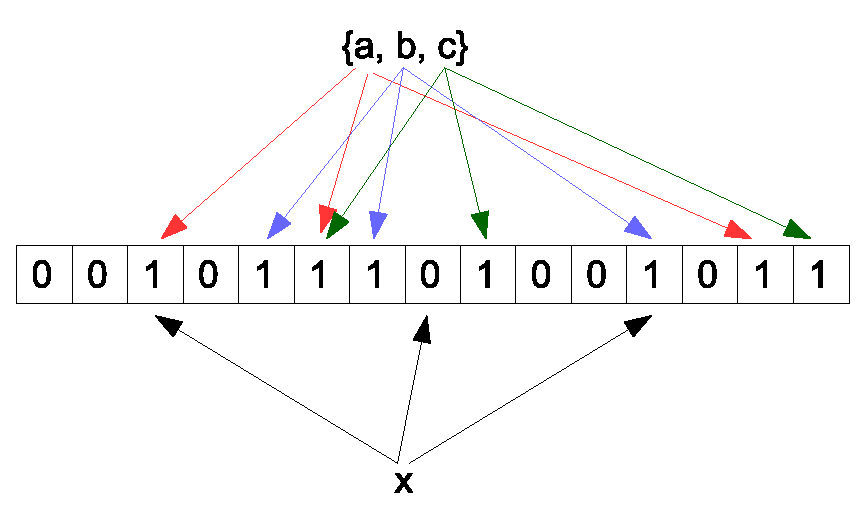
\includegraphics [width=0.6\textwidth]{images/BloomFilter}
  \caption{The inner state and requests to the Bloom filter.}
  \label{fig:bloom_filter}
\end{figure}

The Bloom filter has three parameters that affect its properties.
$m$ - the size of the filter, i.e. the number of bits in the bitset.
Its variation defines not only memory usage, but also the rate of false positives, because the more bits are in use, the less probability of collisions.
$k$ - the number of hash-functions.
This parameter influences again the rate of error.
If there are too less hash-functions, probability to encounter bits, set to 1 by other value, gets more.
At the same time, if there too many hash-functions, filter gets full faster, and again, probability to meet all 1 grows.
Also this parameter affects speed of request to the filter, because every additional hash-function requires time to compute.
$n$ - the number of values, already inserted into the filter.
This parameter is not inherent for the filter, but has a dynamic nature, because it depends on the statistical properties of the stream.
Nevertheless, it affects filter's behavior and is to consider.

Next expression describes the rate of false positives as a function of all three parameters discussed

$$
FP\_rate = \Bigg(1 - \Bigg[1 - \frac{1}{m}\Bigg]^{kn}\Bigg)^k \approx \Big(1 - e^{-kn/m}\Big)^k
$$

Having set parameters $m$ and $n$ we can infer the optimal number of hash-functions, that minimizes error rate

$$
k = \frac{m}{n}ln2
$$

Bloom filter is a great algorithm that finds many examples of use.
Early UNIX spell-checkers used the Bloom filter to check spelling fast, prestoring the whole dictionary in the filter \cite{BroderMitzenmacher2005}.
The Bloom filter allows to store all unsuitable passwords, that users are not permitted to choose \cite{BroderMitzenmacher2005}.
Bitcoin uses the Bloom filter to speed up wallet synchronization \cite{BitcoinFoundation2012}.
Google BigTable and Cassandra systems use the Bloom filter to reduce the number of hard disk lookups \cite{Bigtable/Chang_Dean_Ghemawat}.

\subsection{Count-Min Sketch}

The Count-min sketch answers the query ``how many times has an item been observed in the stream?'' \cite{Cormode}.
It gives always estimated value of the number of occurrences of a particular item.
The rate of error is again a matter of adjusting parameters.
The Count-min sketch can only overestimate the result, meaning give a value equal or greater than true frequency.

The Count-min sketch consists of several arrays of counters.
We denote the matrix, that represents it, as $C$.
Matrix $C$ has $d$ rows and $w$ columns.
The number of rows $d$ is at the same time the number of used hash-functions, so that one function corresponds to one row.
The number of columns $w$ is simply a length of the sketch, and it influences accuracy of the algorithm.

The Count-min sketch works in the following way.
When new item $i$ arrives from the stream, sketch computes each hash-function $h_j(i)$.
For $j$-th hash-function it increments the counter (with index equal to $h_j(i)$) in the $j$-th row of the matrix $C$.
So for each item $i$ sketch increments exactly $d$ counters.
Finally, entry of the matrix $C$ has the next form

$$
C[j, k] = \sum_{h_j(i)=k}f(i)
$$

where $f(i)$ is a frequency of an item $i$.
You can see the view of the Count-min sketch on the Figure ~\ref{fig:count_min_sketch}

\begin{figure}[h]
  \centering
  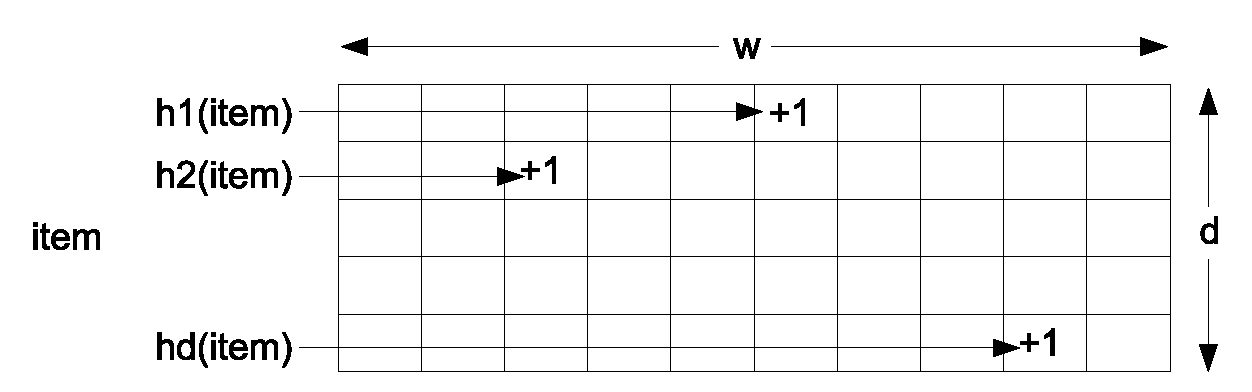
\includegraphics [width=0.6\textwidth]{images/CountMinSketch}
  \caption{The view of the Count-min sketch.}
  \label{fig:count_min_sketch}
\end{figure}

To execute a query, sketch computes again all hash-functions of interesting item $i$, finds all counters, and takes the minimum among them.
As long as collisions can occur, sometimes different items from the stream lead to grow of the same counter in the same row of the matrix.
This can consequently give an overestimation of frequency.
We can reduce the probability of overestimation and its value increasing parameters $d$ and $w$.
The next expression shows frequency estimation for an item

$$
\hat{f}(i) = min_{1 \leq j \leq d}C[j,h_j(i)]
$$

%\subsection{HyperLogLog algorithm}

%The HyperLogLog algorithm answers the query ``how many distinct items have been observed in the stream?''.
%\cite{Heule2013, Flajolet2007}



\section{Anomaly Detection Algorithms [SP]}
\label{sec:anomaly_detection_algorithms}

% [Anomaly Detection : A Survey]
\mnote{anomaly}
\textit{Anomaly} is the data that does not correspond to any expected data patterns.
The presence of anomalies in a data flow can be a sign that something has happened with a source of data.
For example, anomalies are caused by malicious software that changes the system behavior. 
Anomalies in data, collected from medical sensors, can indicate the drastic changes in a patient state of health.
Moreover, an anomaly in sensor data can be a forerunner of a catastrophe, like flood or even a nuclear power plant crash.
Therefore, it is necessary to use an anomaly detection mechanism to prevent undesirable situations.

It is important to distinguish between \textit{anomaly}, \textit{noise} and \textit{novel data} \cite{Chandola2007}.
Noise is a deviation from normal patterns, that is not interesting for analysis.
Ideally all the noise should be removed before analyzing the information.
Novel data appears when the pattern changes.
This data arrives continuously and leads to creation a new pattern that is later included into the normal model.  

Anomaly detection process is accompanied by the following difficulties.
Usually it is difficult or event not possible to name all the patterns that correspond to the normal behavior.
The boundary between normal and anomalous data can be uncertain.
The behavior that is considered to be normal can change in the course of time.
It is necessary to get rid of noise, that can look like anomalies in some cases.
The degree of deviation from the normal behavior can be different in different situations.
Sometimes anomaly differs from the expected pattern slightly, while in other case the difference can be huge.
Finally, the malicious software often tries to imitate the normal behavior to obstruct its detection. 

\mnote{types of anomaly}
Anomalies can be divided into three categories \cite{Chandola2007}.
The simplest one is a \textit{point anomaly}.
It is an individual instance that differs from all other instances in a given data flow.
Most of the time anomaly detection works with this category of anomalies.
The second one is a \textit{contextual anomaly}.
In this case the instance is analyzed taking into account its neighboring instances.
It means that if such data instance occurs without a particular context, it is not considered to be an anomaly.
The third category is a \textit{collective anomaly}.
It appears only when the data instances in a data set are related to each other.
For example, a collective anomaly is an appearance of the same data instance in a row, while usually they should be separated by other instances.

\mnote{supervised approach}
Different approaches of anomaly detection exist.
They are grouped into three types: supervised, semi-supervised and unsupervised approaches.
For using a supervised mode, one needs two labeled sets: the normal data and anomalous data.
If a system receives an unlabeled instance, it compares this instance to existing classes and makes a prediction to which class it belongs to.
The problem with supervised approach is that usually the anomalous data set is much smaller than the normal one.
Moreover, as anomaly occurs accidentally, it is not possible in some cases to have representative labels for this class of instances.
 
\mnote{semi-supervised approach}
The semi-supervised anomaly detection is almost the same as the supervised, with the exception that it has labels only for the normal instances.
In this case the received data is compared to existing normal pattern and the conclusion is made whether this instance is an anomaly or not.
Theoretically it is possible to use such technique vice versa, having the labels only for anomalous data.
However, often it is hard to predict all the anomalies that can occur in a given system.

\mnote{unsupervised approach}
The unsupervised approach does not need a predetermined data classes.
This technique is based on the assumption that anomalies occur rarely, comparing to the normal data instances.
Because this approach does not use a training set, it is the most popular anomaly detection mechanism.
This assumption makes possible to adapt a semi-supervised way to an unsupervised one.
For this purpose all the available data is labeled as a normal class.

From the practical side multiple techniques are used for anomaly detection:
(1) Classification based, (2) Nearest neighbor based, (3) Clustering based, (4) Statistical, (5) Information theoretic, (6) Spectral.
Each of them has its own advantages and disadvantages and is better suited for different data sets.
Several most widespread techniques are described in the following paragraphs.

\mnote{classification based anomaly detection}
Classification based anomaly detection uses a training data set to learn a model.
Then a trained model works as a classifier, assigning a newcomer data instance a label 'normal' or 'anomaly'.
Classification based technique can be multi-class or one-class.
Multi-class case implicates multiple normal classes.
A classifier detects which normal class a new data instance belongs to.
If it does not belong to any, it is considered to be an anomaly.
One-class technique has the same logic, except that in this case there is only one normal class.

\mnote{neural network}
One can use various machine learning algorithms to implement classification based anomaly detection.
An example of such algorithm is a neural network based approach.
In the first phase, the neural network is learned using a labeled training set. 
In the second phase, the network receives an unlabeled instance and accepts or rejects it.
In the case of rejection the instance is considered an anomaly.

\mnote{Bayesian network}
Another algorithm is a Bayesian network based approach.
It works on an estimation of the posterior probability that the data instance belongs to one of the given classes.
The class label that has the greatest posterior probability is assigned to an observed data instance.

\mnote{SVM}
One more algorithm in classification based category is Support Vector Machines (SVM).
In this case the result of learning is a region.
If a test instance falls into this region - it is normal, if not - it is an anomaly.

\mnote{rule based}
The last algorithm in this category is rule based.
In the first phase the rules are created from the test data.
In the second phase the rule is chosen that is best suited for a given data instance. 
A well-known example of such algorithm is Decision Trees.

The advantage of classification based approaches is that the data model is pre-computed.
It means that the new unlabeled data instance can be immediately compared to the existing model and became classified.
The main drawback is that sometimes it is difficult or not possible to put labels on all normal classes.

\mnote{nearest neighbor based anomaly detection}
The next technique is nearest neighbor based anomaly detection.
The main concept of this method is a distance metric between data instances.
It is assumed that anomalies are situated far from other instances in a feature space.

Nearest neighbor techniques consist of two groups depending on how the anomaly score is computed.
On the one hand, it is possible to calculate the distance between a data instance and its neighbors.
On the other hand, one can find a relative density of a data instance to detect anomalies.

The main attraction of nearest neighbour methods is that they are unsupervised.
There is no need in labeling data instances, these methods are data driven.
The drawback is that such technique works only for those data sets, where normal data instances have many close neighbors, while anomalies have few neighbors.
Moreover, it has a problem with computation complexity.
As it is necessary to calculate distances to all the instances, it usually takes $O(N^2)$ time.
The performance can be improved by using k-d trees or R-trees for searching nearest neighbors.

\mnote{clustering based anomaly detection}
In the case of clustering based anomaly detection all the data is grouped into clusters.
There are three ways how clustering can be used.
First approach assumes that the data instances that are not belong to any clusters can be considered as anomalies.
An example of such clustering algorithm is DBSCAN, that allows instance to be an outlier that does not belong to any cluster.
Second approach considers the instances as anomalies when they are far from cluster centroids.
For instance, K-means clustering can be used in this case.
Third, when anomalous data instances also compose clusters, the distinction between cluster size or density serves as a dividing factor.

The clustering based technique differs from the nearest neighbor based one in that in the former case a data instance depends on the cluster it belongs to, while in the latter case the neighborhood of the data instance influence on its evaluation.

Clustering based anomaly detection also gives an advantage of operating in an unsupervised mode.
Another positive side is testing phase performance.
As the number of clusters is limited, the algorithm works fast.
The disadvantage of this technique is that clustering initially designed to form clusters from data set and anomaly detection is only a by-product of the algorithms.

\mnote{statistical anomaly detection}
Statical technique constructs a statical model and tests whether a new data instance belongs to it or not.
There are two types of statical methods: parametric and non-parametric.
The former one assumes that the distribution of processed data is known, while the latter does not know about the underlying distribution.

Parametric methods include techniques, that based on various distributions.
For example, the data can be distributed according to Gaussian law.
In this case the anomaly score is the distance between estimated mean and the data instance.
Another parametric method is a regression model based technique.
Moreover, there is a possibility to use several statistical distributions in one technique.

Non-parametric techniques construct a data model from given data.
For instance, histogram based method creates a histogram that reflects the normal data values.
If a new data instance cannot be put in any bin of the histogram, it is labeled as anomaly.

Statistical anomaly detection techniques do not need labeled data for training, so they run in an unsupervised mode.
Another benefit is that when the distribution law works for given data, the detected anomaly can be statistically justified.
However, usually it is a difficult task to find a proper statistical model.

\mnote{information theoretic anomaly detection}
Information theoretic way is based on information content analysis of given data.
It assumes that anomalies increase entropy of the information content.
Along with entropy, other measures like relative entropy or Kolomogorov Complexity are used.

\mnote{spectral anomaly detection}
Spectral anomaly detection methods try to find subspaces, where normal and anomalous data is easy distinguishable.
For example, projections or embedding can be used to create such subspaces.
Therefore such techniques can work with high dimensional data.
The drawback of spectral analysis is its high computational complexity.   
%\section{Application in the speed layer}

Descirbe how stream processing algorithms can be applied in the speed layer.
How can we build topology to solve some particular task, to creat some aggreagation for example.
How all this works technically, data pipelines, usage of different algorithms.